\documentclass[letterpaper]{article}
% Required Packages
\usepackage{aaai}
\usepackage{times}
\usepackage{helvet}
\usepackage{courier}
\usepackage{changepage}
\usepackage{graphicx}
\usepackage[noend]{algpseudocode}
\usepackage{subcaption}
\graphicspath{ {/afs/inf.ed.ac.uk/user/s09/s0954584/Dropbox/4th/unshredder/writing/imgs/} }
\setlength{\pdfpagewidth}{8.5in}
\setlength{\pdfpageheight}{11in}
%%%%%%%%%%
% PDFINFO for PDFLATEX
% Uncomment and complete the following for metadata (your paper must compile with PDFLATEX)
\pdfinfo{
/Title (A Modular Framework for the Automatic Reconstruction of Shredded Documents)
/Author (Razvan Ranca)
/Keywords (shredded, document, reconstruction, strip-cut, cross-cut, unshred, deshred)
}
%%%%%%%%%%
% Section Numbers
% Uncomment if you want to use section numbers
% and change the 0 to a 1 or 2
% \setcounter{secnumdepth}{0}
%%%%%%%%%%
% Title, Author, and Address Information
\title{A Modular Framework for the Automatic Reconstruction of Shredded Documents}
\author{Razvan Ranca\\
School of Informatics, University of Edinburgh\\
10 Crichton Street, Edinburgh, Scotland, United Kingdom\\
\emph{ranca.razvan@gmail.com}
}
\nocopyright
%%%%%%%%%%
% Body of Paper Begins
\begin{document}
\maketitle

\begin{adjustwidth}{10pt}{10pt}
\section{
\fontsize{10pt}{12pt} 
\selectfont 
Abstract}

\fontsize{9pt}{10pt}
\selectfont
The unshredding problem is of interest in various domains such as forensics, investigative sciences and  archeology, and has therefore been approached in many different ways. This paper tries to bridge the gap between previous, disparate, efforts by proposing a modular, probabilistic, solution. Novel approaches to two of the independent subproblems are presented and shown to both have good theoretical properties and to empirically outperform previously published methods.
\end{adjustwidth}

\section{
\fontsize{12pt}{15pt} 
\selectfont
Introduction}
\fontsize{10pt}{12pt} 
\selectfont
The US Federal Trade Commission recommends the shredding of sensitive documents as a good protection method against becoming one of the millions of victims of identity theft\footnote{http://consumer.ftc.gov/features/feature-0014-identity-theft}. However, the successfully solved DARPA Shredder challenge\footnote{http://archive.darpa.mil/shredderchallenge/} and the appearance of commercial document reconstruction services\footnote{eg: http://www.unshredder.com/}, puts the security of the shredder into question. Further research in this area will benefit projects such as the ongoing effort to recover the shredded archives of the East German secret police, which consist of 16,000 bags of shredded documents. Since it took 3 dozen people 6 years to reconstruct 300 of these bags \cite{P6}, at this rate, the project would require 11,520 person-years.

The unshredding challenge can be approached by splitting the problem into three independent subproblems. A \emph{pre-processing} step transforms the noisy images of scanned shreds into uniform ``ideal shreds". A \emph{scoring function} then evaluates the potential match between every pair of shreds and, finally, a \emph{search method} finds the permutation of shreds that obtains a good global score. In this paper I present a novel, composable, probabilistic scoring function and an original, graph-inspired, search heuristic which balances speed and accuracy while achieving modularity.

\section{
\fontsize{12pt}{15pt} 
\selectfont
Related Work}
\fontsize{10pt}{12pt} 
\selectfont
Significant effort has been made towards finding a good search function. \cite{P1} show that the search is NP hard by reduction to the Traveling Salesman Problem. \cite{P2} attempts an Integer Linear Programming solution which yields good results but is intractable for more than 150 shreds. \cite{P3,P4} try instead to formulate the search as an evolutionary algorithm. 

In contrast, relatively little progress has been made in developing the score function. All previously mentioned papers settled on a formulation which selects a score based on a weighted difference of the adjacent pixels on either side of the proposed join. \cite{P7} provides a formal definition. 
\cite{P5} refine this method by placing an emphasis on black pixels, thus discounting the information content of white pixels. \cite{P8} try a different approach, by employing optical character recognition techniques. Their method is however left as a proof-of-concept, since it is not integrated with a search function or evaluated against any other scoring methods.

Finally, pre-processing can be split into several independent functions, which have been previously explored. For instance, \cite{P9} extracts the shreds from scanned input images via rectangle and polynomial fitting, while \cite{P10} fix the skew of the extracted shreds by framing the issue as an optimization problem. Up/down orientation of documents is explored in \cite{P11,P12} with good results, though the methods are only evaluated on full documents, not shreds.
\section{
\fontsize{12pt}{15pt} 
\selectfont
Probabilistic Score}
\fontsize{10pt}{12pt} 
\selectfont
I propose a novel score function formulation, which uses a probabilistic model to directly estimate the likelihood of two edges matching. Employing a probabilistic model offers several advantages, such as an increase in robustness given by the ability to train the model on the document shreds and easy composability of different models, simply achieved by multiplying their probabilities and re-normalizing.

I test this idea by implementing a basic probabilistic model, based on the conditional probability that a pixel is white or black given a few of its neighboring pixels. Formally, given edge \emph{Et}, \emph{ProbScore} returns the best match for Et and the probability of that match. ProbScore is defined:
\begin{algorithmic}
\Procedure {ProbScore}{$Et$}
  \State {Initialize $ps$} \Comment{\emph{probabilities of matches, initially all 1}}
  \ForAll{$Ex \in Edges$} 
    \ForAll {$pixel \in Ex$}
      \State $ps_{Ex} \gets ps_{Ex} * \Pr(pixel|Neighbors_{Et}^{pixel})$ 
    \EndFor
  \EndFor
  \State {Normalize $ps$} \Comment{\emph{probabilities must sum up to 1}}
  \State \textbf{return} $\arg\max ps$, $\max ps$
\EndProcedure
\end{algorithmic}

Empirical results show that this probabilistic score compares favorably to the most common scoring function used in literature \cite{P7}, both on noise-less documents and on several noisy documents. Additionally, in order to showcase the benefits offered by the modular nature of ProbScore, I compose it with another probabilistic model called \emph{RowScore} which applies a Gaussian model to the distance between rows in neighboring shreds. Even such a simple model gives ProbScore a small but consistent boost (see Figure \ref{fig:scoreComp}). ProbScore could also be composed with more complex models, such as that proposed by \cite{P8}.
\begin{figure}[h]
%\setlength{\textfloatsep}{0pt plus 1.0pt minus 2.0pt}
%\setlength{\floatsep}{0pt plus 1.0pt minus 2.0pt}
\setlength{\abovecaptionskip}{8pt plus 1.0pt minus 2.0pt}
%\setlength{\belowcaptionskip}{0pt plus 1.0pt minus 2.0pt}

    \centering
    \begin{subfigure}[b]{0.23\textwidth}
        \setlength{\abovecaptionskip}{4pt plus 1.0pt minus 2.0pt}
        \centering
        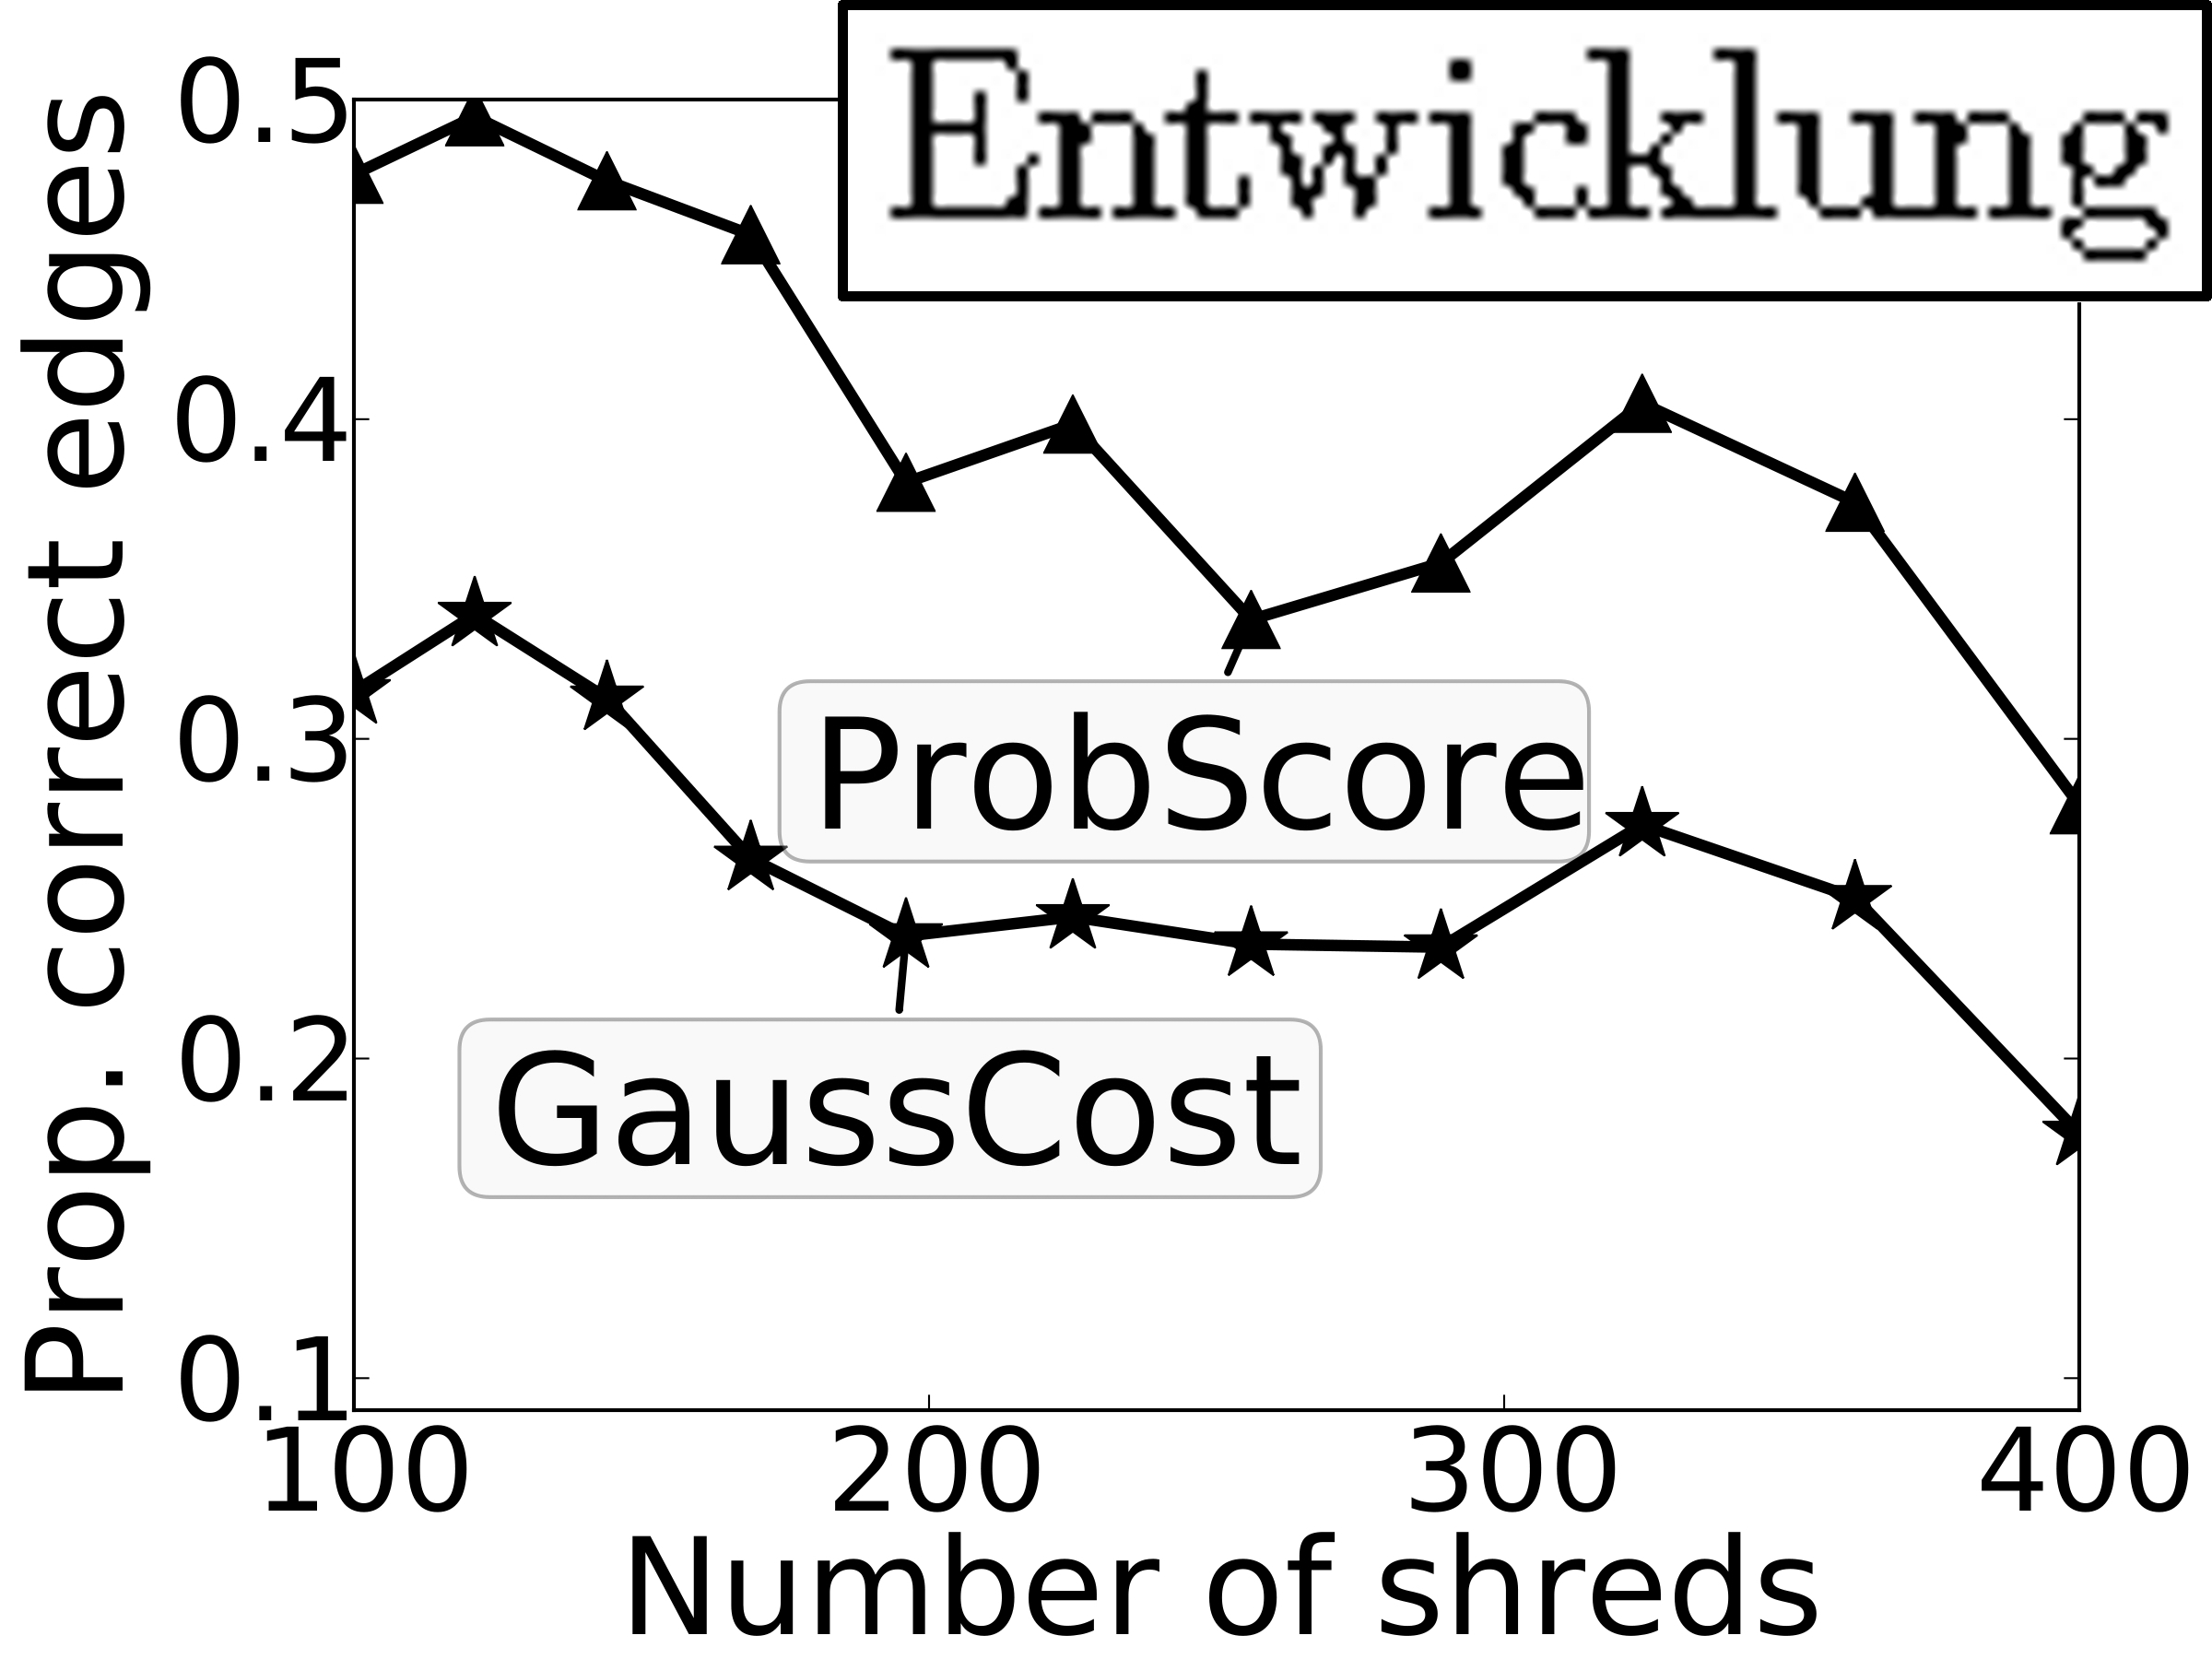
\includegraphics[width=\textwidth,height=3cm,natwidth=610,natheight=642]{origCompBWEnt.jpg}
        \caption{Original document.}
    \end{subfigure}
    \begin{subfigure}[b]{0.23\textwidth}
        \setlength{\abovecaptionskip}{4pt plus 1.0pt minus 2.0pt}
        \centering
        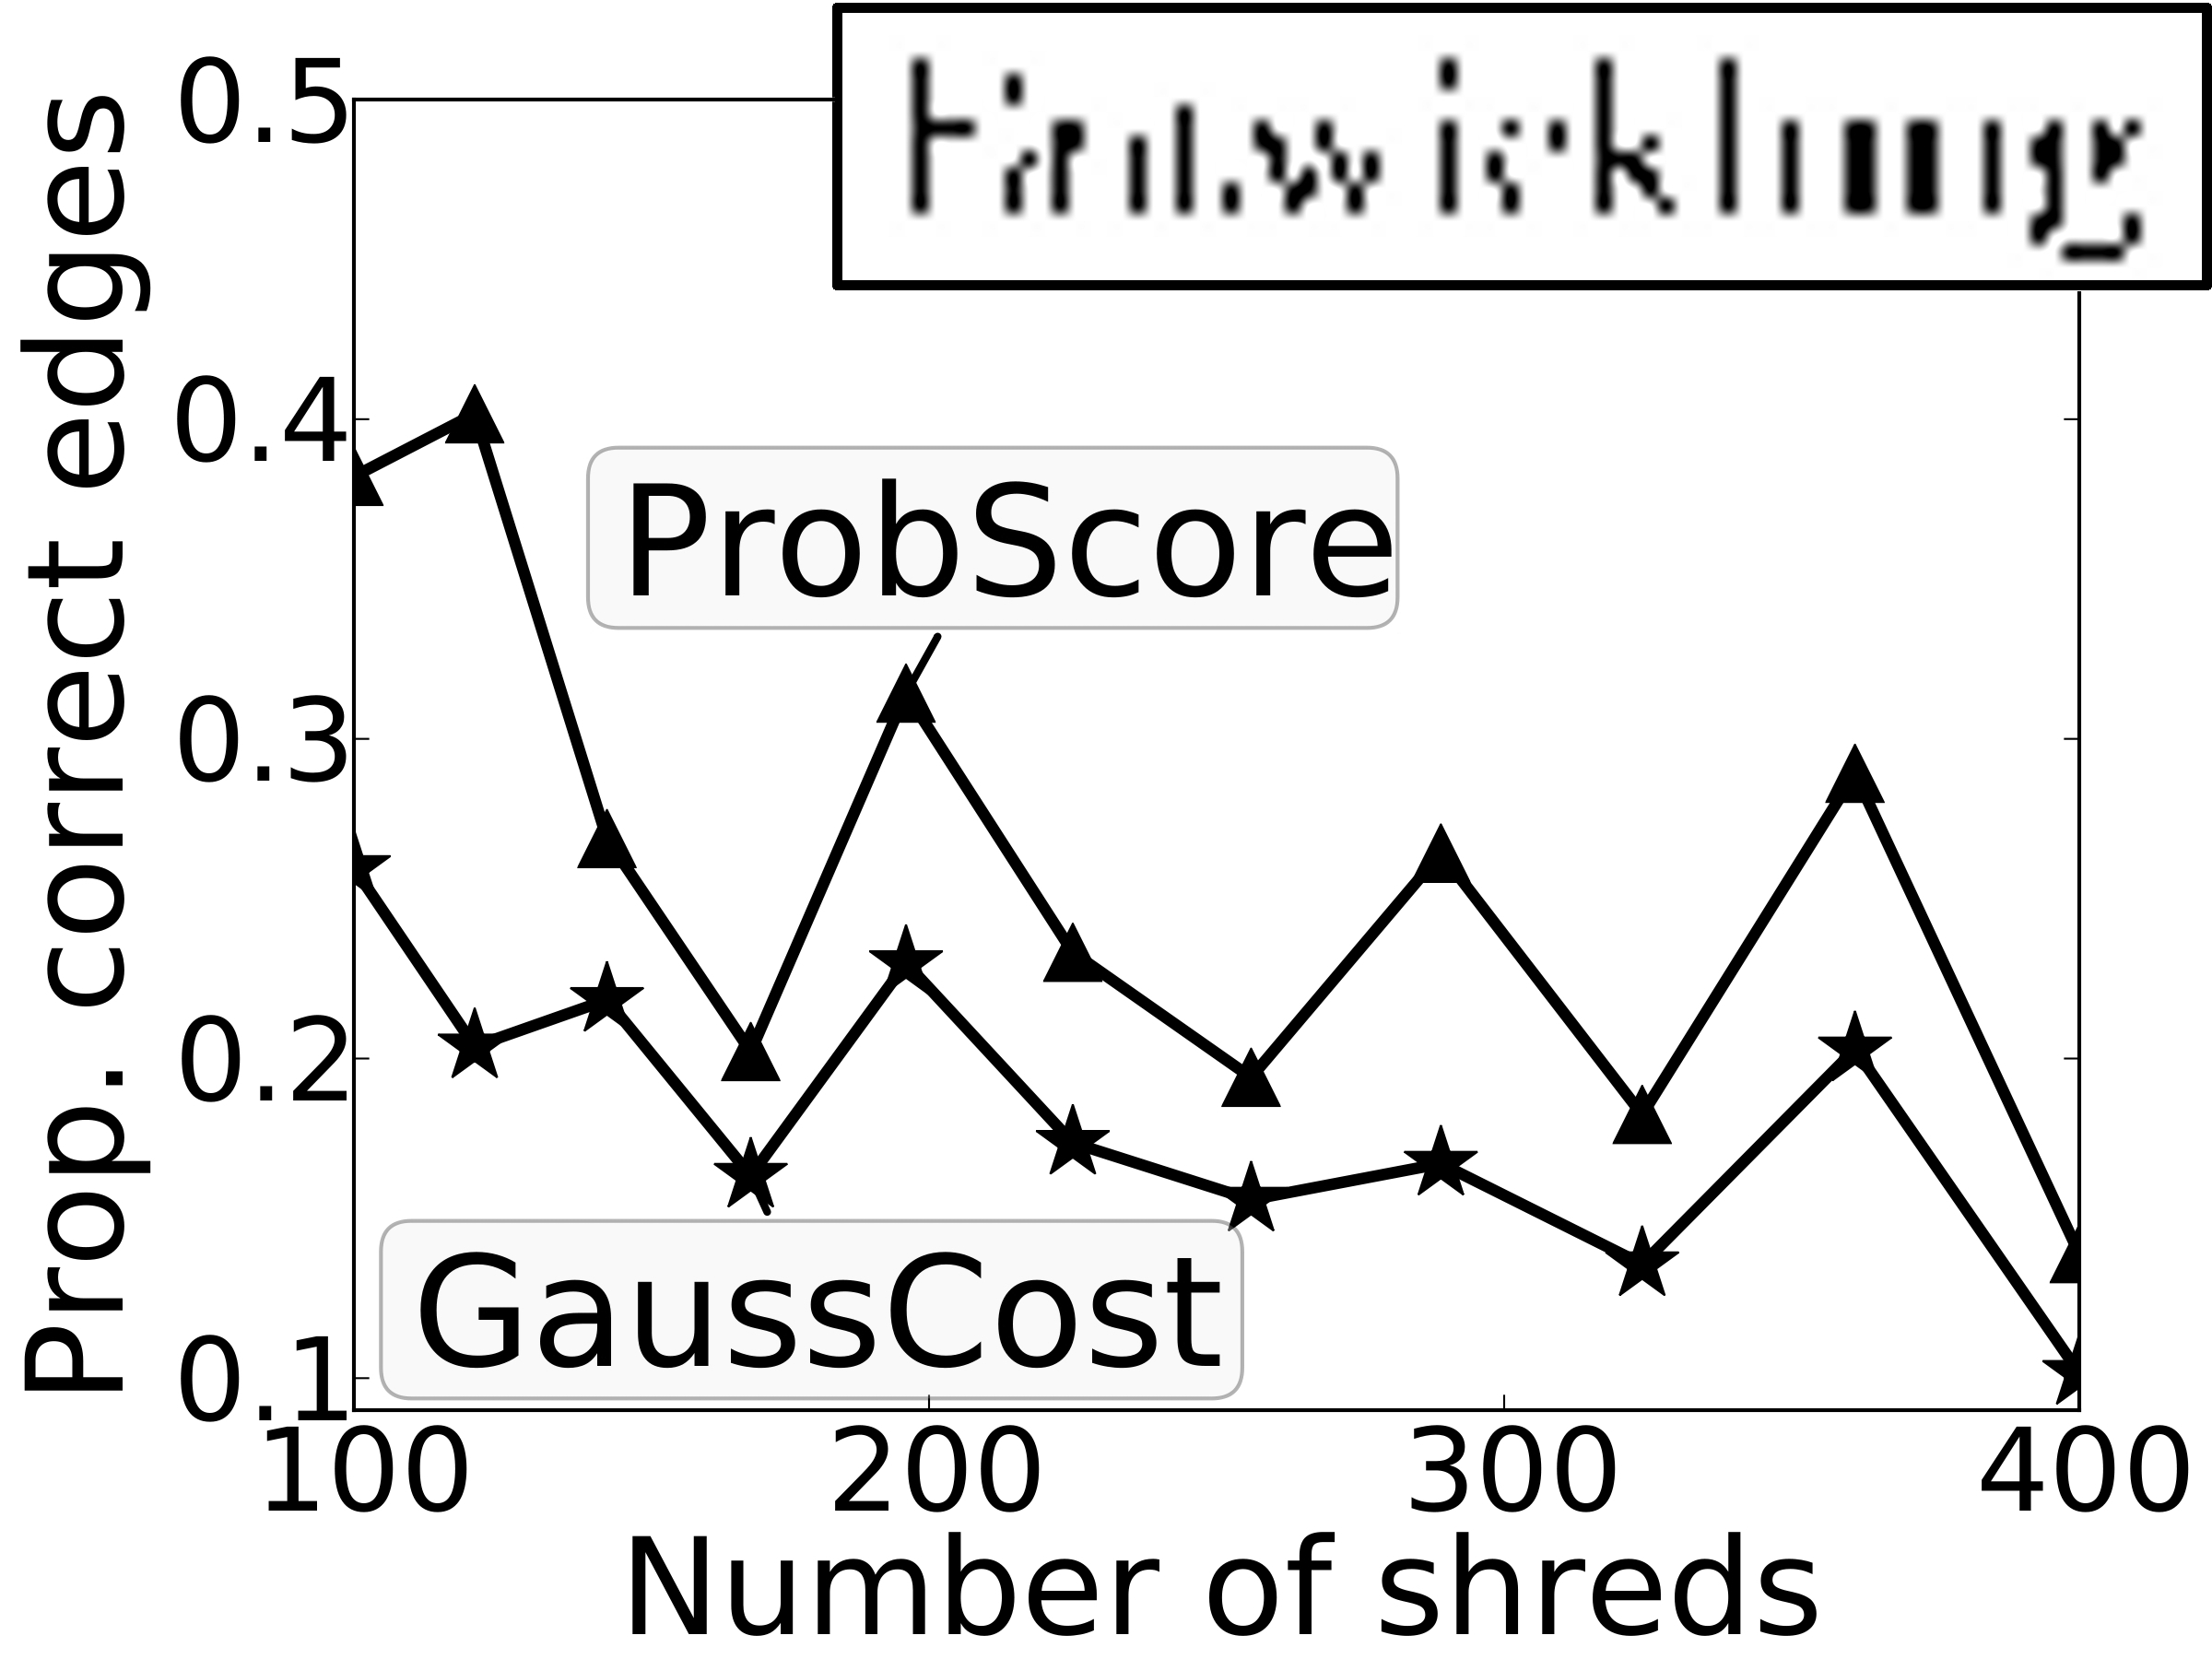
\includegraphics[width=\textwidth,height=3cm,natwidth=610,natheight=642]{downsampleBWEnt.jpg}
        \caption{Downsampled document.}
    \end{subfigure}
    \begin{subfigure}[b]{0.23\textwidth}
        \setlength{\abovecaptionskip}{4pt plus 1.0pt minus 2.0pt}
        \centering
        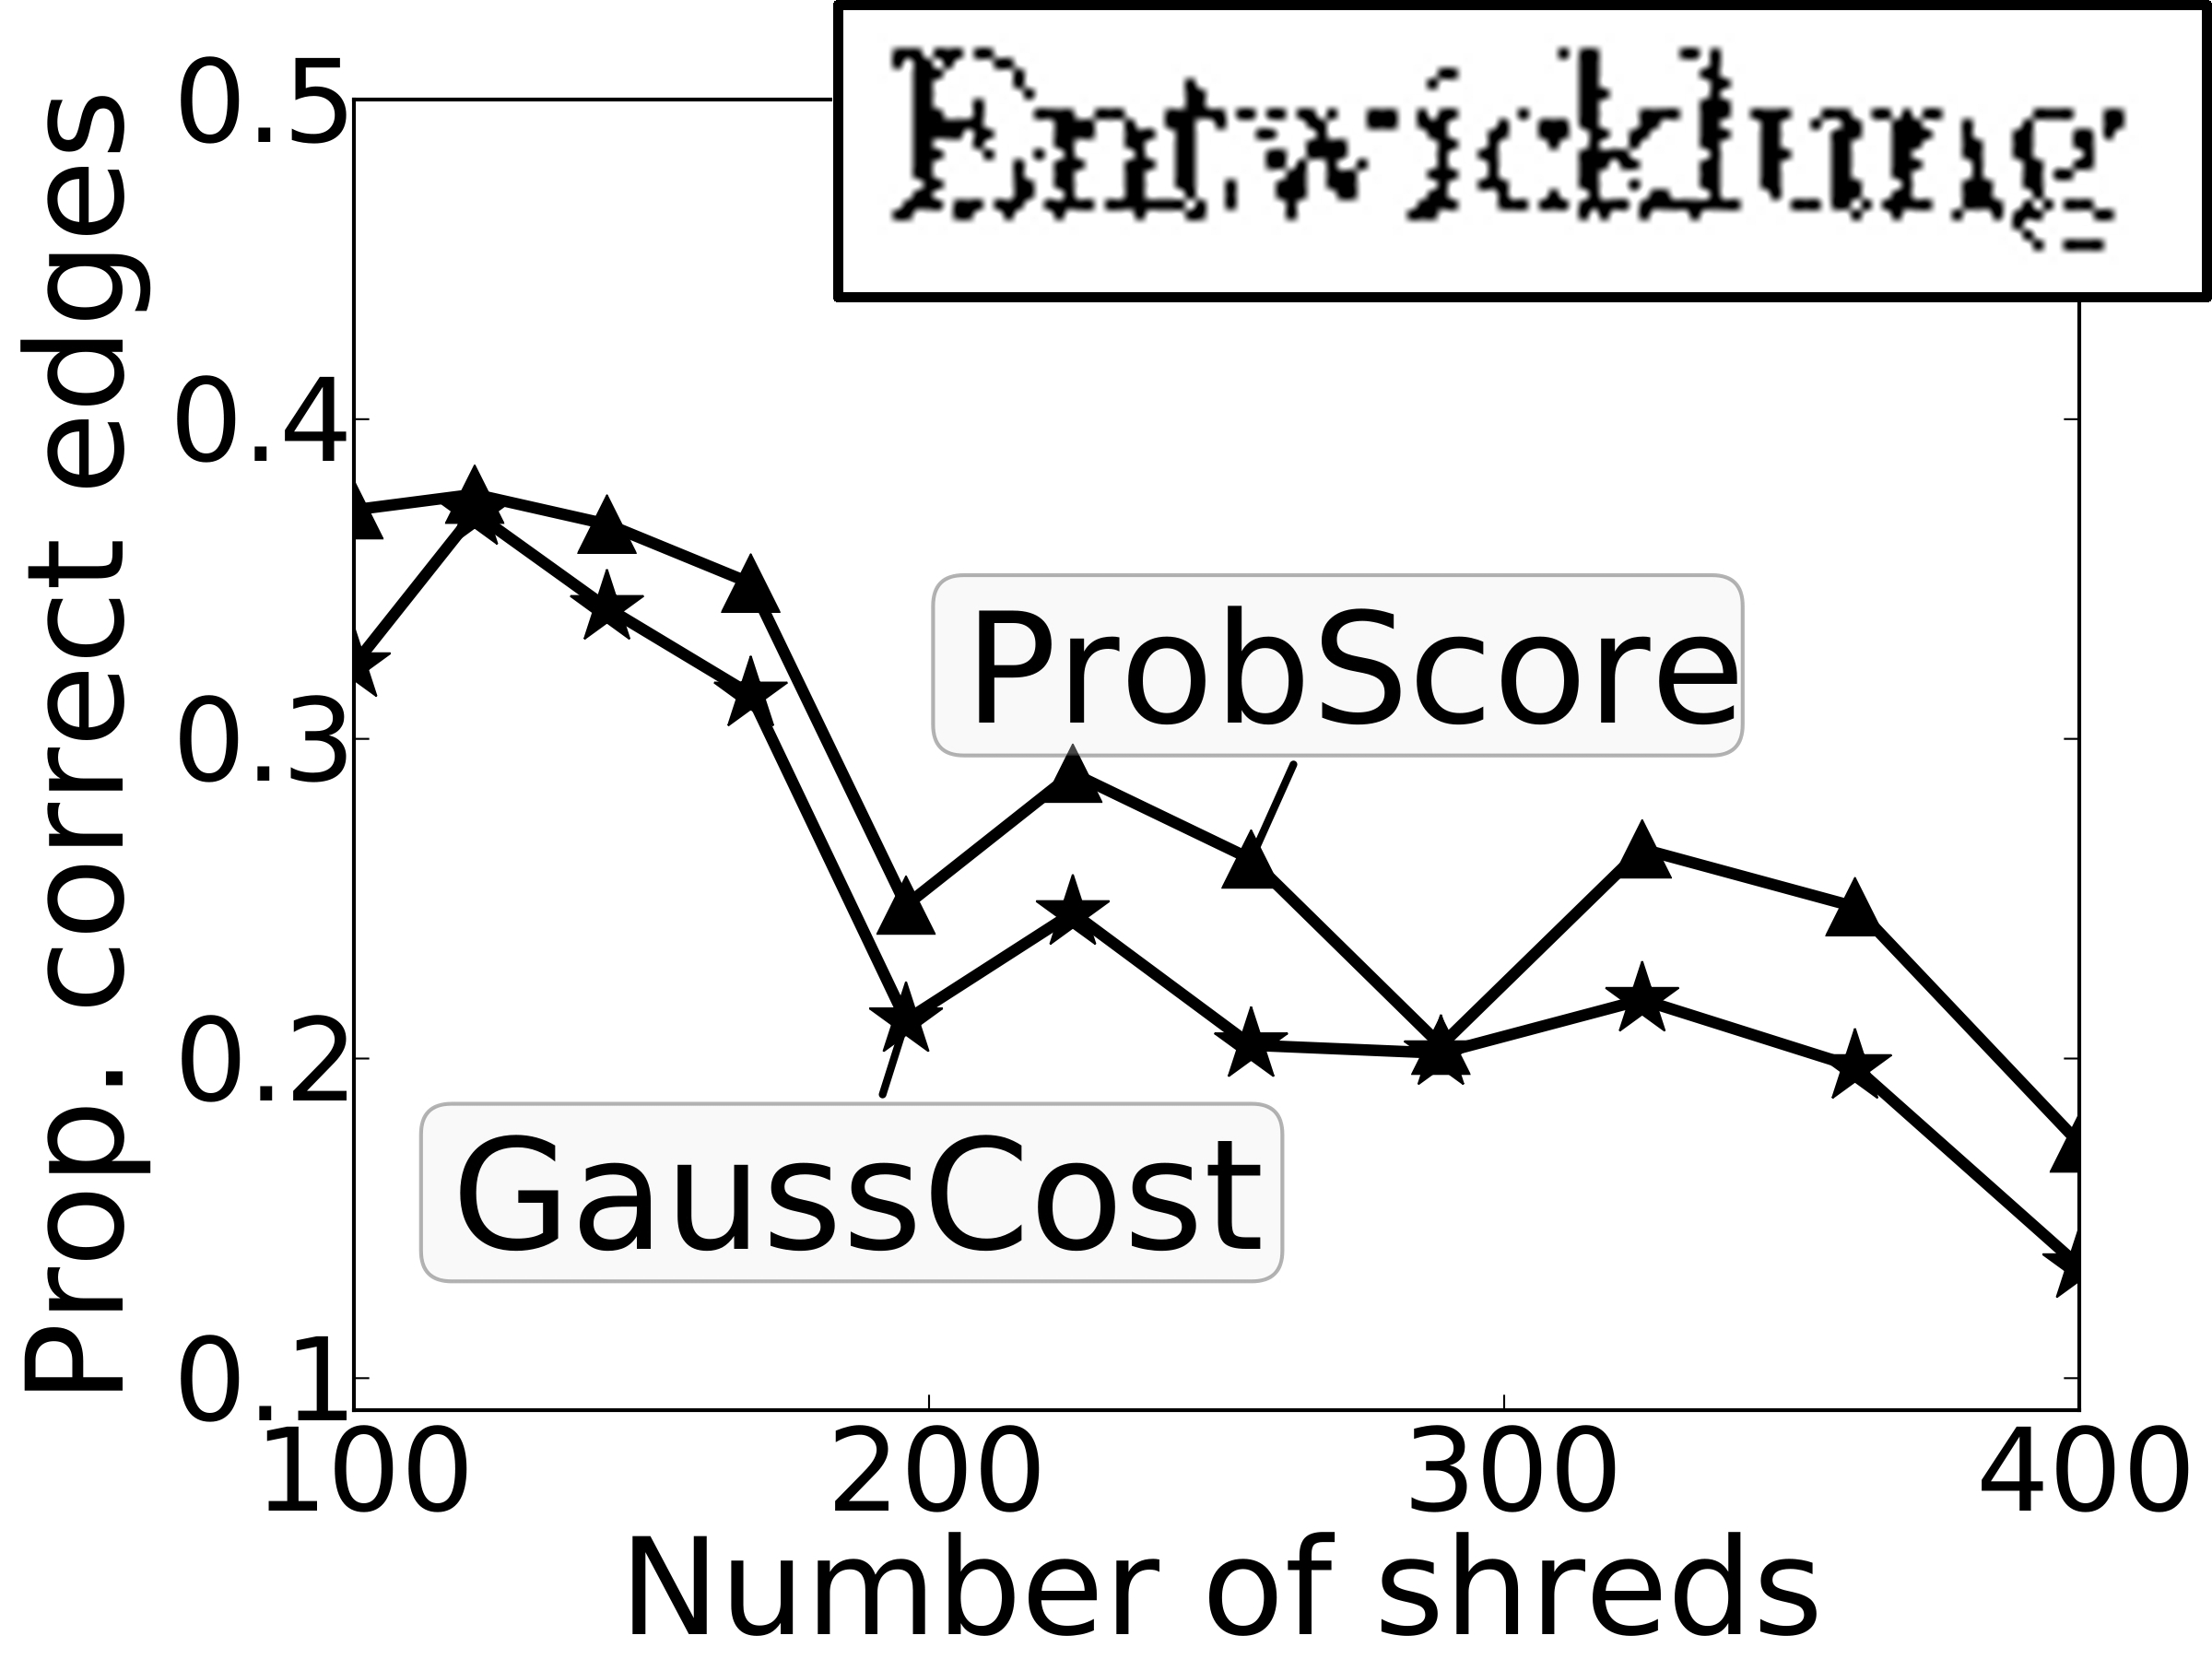
\includegraphics[width=\textwidth,height=3cm,natwidth=610,natheight=642]{shuffleBWEnt.jpg}
        \caption{Noisy document.}
    \end{subfigure}
    \begin{subfigure}[b]{0.23\textwidth}
        \setlength{\abovecaptionskip}{4pt plus 1.0pt minus 2.0pt}
        \centering
        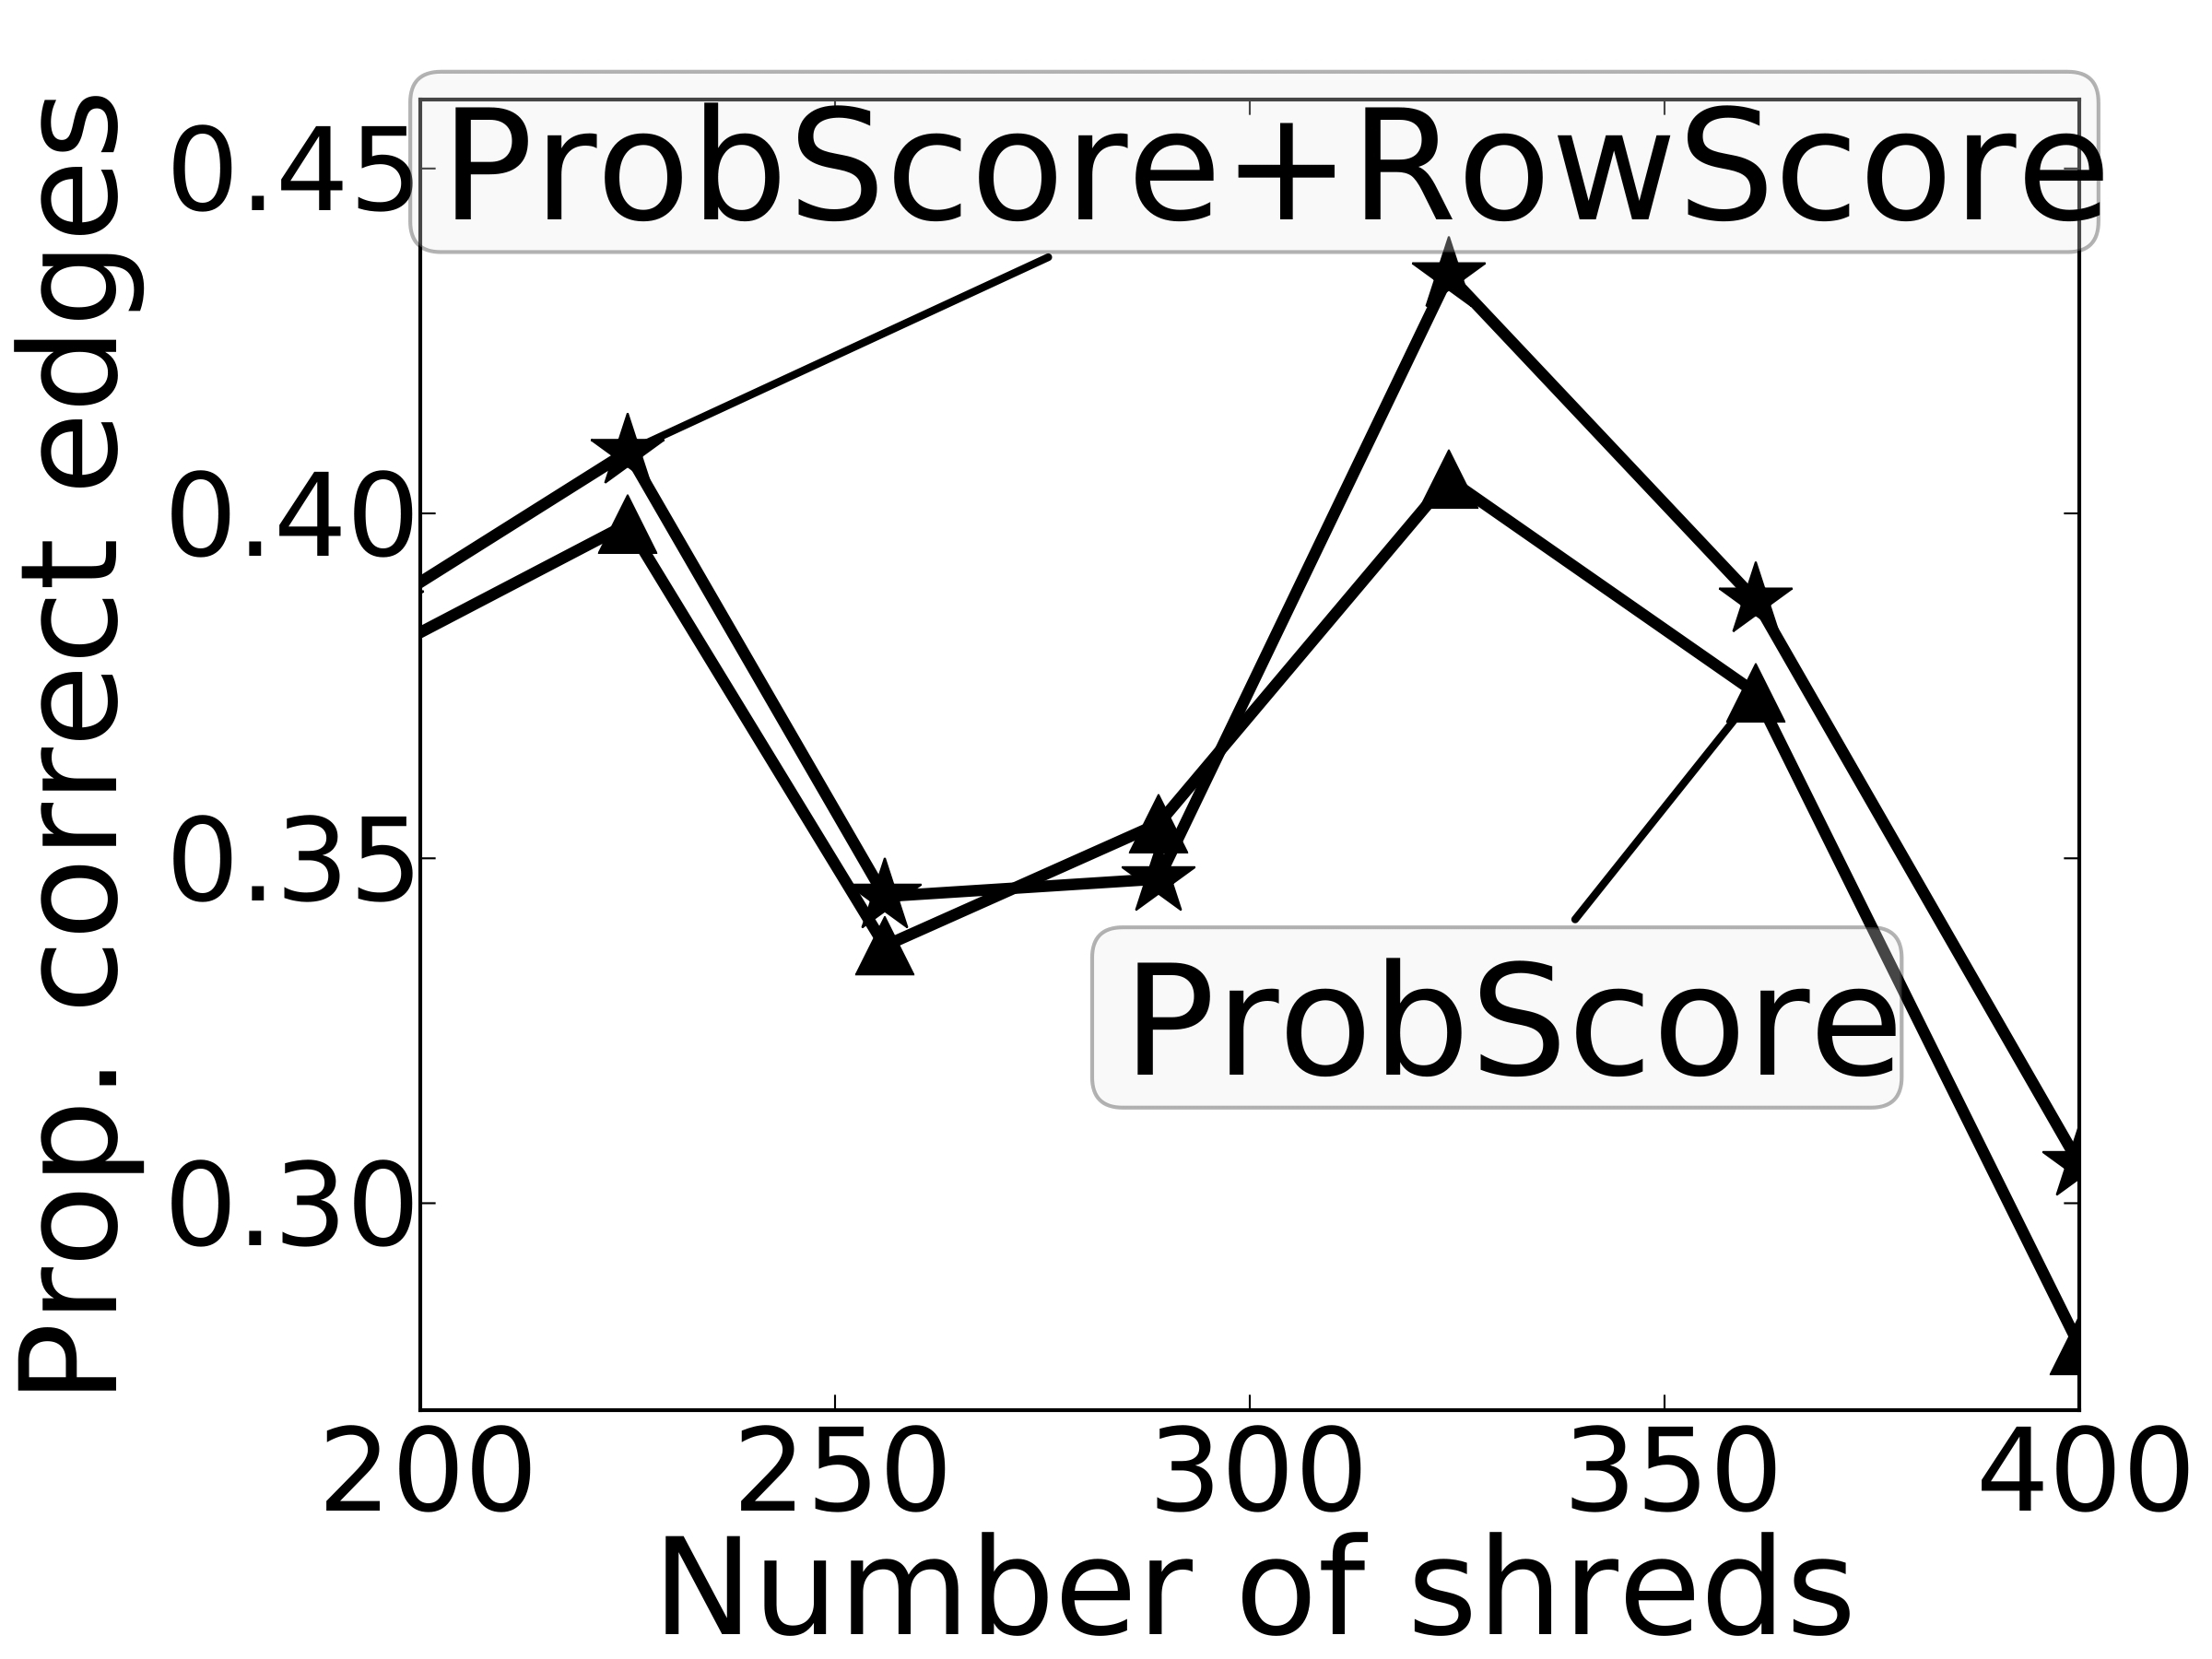
\includegraphics[width=\textwidth,height=3cm,natwidth=610,natheight=642]{rowCompBW.jpg}
        \caption{Score function composition.}
    \end{subfigure}
     \caption{Figures {\bf a},{\bf b} and {\bf c} show comparisons between our method and the most common previously used function. A sample word from each document is shown in the upper right corners. Figure {\bf d} shows the improvement obtained by composing our function with another probabilistic model.}
    \label{fig:scoreComp}
\end{figure}

\section{
\fontsize{12pt}{15pt} 
\selectfont
``Kruskal-Inspired" Heuristic Search}
\fontsize{10pt}{12pt} 
\selectfont
Extending the heuristic introduced in \cite{P5}, I implement a search method inspired by the minimum spanning tree ``Kruskal's algorithm" \cite{P13}. The method greedily picks the most probable edge and tries to match the two shreds along that edge. This process creates multiple clusters of shreds which will eventually be merged into a single solution. Before performing a merge, I check if the move would result in two shreds being superimposed, in which case the merge is aborted.

This method outperforms previously proposed bottom-up heuristics but is still significantly more tractable than any of the top-down optimizing search functions. A novel aspect of the heuristic is that, if the next move is uncertain, execution can be stopped. This functionality achieves my overarching goal regarding modularity, since it means the method can reduce the search space of a problem, such that a more complex search function may become feasible (see Figure \ref{fig:searchRez}).

\begin{figure}[h]
%\setlength{\textfloatsep}{0pt plus 1.0pt minus 2.0pt}
%\setlength{\floatsep}{0pt plus 1.0pt minus 2.0pt}
\setlength{\abovecaptionskip}{1pt plus 1.0pt minus 2.0pt}
%\setlength{\belowcaptionskip}{0pt plus 1.0pt minus 2.0pt}

    \centering
    \begin{subfigure}[b]{0.48\textwidth}
        \setlength{\abovecaptionskip}{0pt plus 1.0pt minus 2.0pt}
        \centering
        
\includegraphics[width=\textwidth,height=1.9cm,natwidth=610,natheight=642]{prim7x7BW.jpg}
        \caption{Cross-cut document output.}
    \end{subfigure}
    \begin{subfigure}[b]{0.23\textwidth}
        \setlength{\abovecaptionskip}{0pt plus 1.0pt minus 2.0pt}
        \centering
        
\includegraphics[width=\textwidth,height=4.9cm,natwidth=610,natheight=642]{prim1x49BW.jpg}
        \caption{Strip-cut document output.}
    \end{subfigure}
    \begin{subfigure}[b]{0.23\textwidth}
        \setlength{\abovecaptionskip}{0pt plus 1.0pt minus 2.0pt}
        \centering
        
\includegraphics[width=0.8\textwidth,height=4.9cm,natwidth=610,natheight=642]{stopped7x7BW.jpg}
        \caption{Cross-cut, stopped at 99.5\%.}
    \end{subfigure}
     \caption{Figures {\bf a} and {\bf b} show full reconstructions on the cross-cut variant (64\% correct) and the strip-cut variant (100\%correct). Figure {\bf c} shows a partial reconstruction (stopped at 99.5\% certainty) which successfully reduces the search space from 49 to 10 shreds while introducing 0 errors.}
    \label{fig:searchRez}
\end{figure}
It's worth noting that cross-cut documents are significantly harder to solve than strip-cut ones. This is due to the short edges produced by cross-cutting, which are harder to model accurately. Horizontal cuts also have a significant chance of falling between two lines of text, in which case the score function has no information on how to order the lines.
\section{
\fontsize{12pt}{15pt} 
\selectfont
Conclusions and Future Work}
\fontsize{10pt}{12pt} 
\selectfont
This paper presents a modular and composable framework for the shredded document reconstruction problem and provides sample solutions for 2 of its 3 components. Specifically, I propose a probabilistic scoring function which outperforms currently used alternatives and a tractable search heuristic which can solve simpler reconstruction problems and reduce the search space for more complex ones.

Future work will look at implementing more advanced score and search functions. Solving the cross-cut domain will likely require scoring functions which employ computer vision techniques and search function which perform a partial exploration of the search tree. The performance of the independent, pre-processing, components will also be tested as the size of their input documents decreases.

%%%%%%%%%%
% References and End of Paper
\bibliographystyle{aaai}
\bibliography{paper}
\end{document}
